\documentclass[conference]{IEEEtran}
\usepackage{graphicx}
\usepackage[]{siunitx}
\DeclareSIUnit[]{\fps}{FPS}
\usepackage[
    %backend=bibtex,
    backend=biber,
    texencoding=utf8,
    bibencoding=utf8,
    style=ieee
]{biblatex}
\addbibresource{main.bib}

\usepackage{booktabs}
\usepackage{cleveref}
% correct bad hyphenation here
\hyphenation{op-tical net-works semi-conduc-tor}

\begin{document}
\title{Face Recognition on the PYNQ platform}


% author names and affiliations
% use a multiple column layout for up to three different
% affiliations
\author{
\IEEEauthorblockN{Erwin de Haan}
\IEEEauthorblockA{4222814\\TU Delft}
\and
\IEEEauthorblockN{Sybold Hijlkema}
\IEEEauthorblockA{4449487\\TU Delft}}
\date{\today}
% make the title area
\maketitle

\section{Introduction}
Face recognition is a very interesting and well researched topic. Algorithms like a haar\_classifier can run real-time facial recognition on modern hardware. On smaller embedded systems this can still be a challenge however. We implement a down-sampling and a out-of-loop face recognition application. The FPGA fabric is used to composite the indicators and send the video frame to the SoC for processing.
In this report facial recognition is used with either only a ARM CPU or with a combination of an FPGA and a ARM CPU.

\hfill \today
\section{Setup}
An FPGA of the Zynq family (XC7Z020) is used which has an ARM SoC on-chip, running the Pynq platform on the PYNQ-Z1 development board, manufactured by Digilent. The FPGA is connected with the HDMI\_IN to a computer and with the HDMI\_OUT to a monitor. The SoC runs a linux distribution and a program written in python.

\section{Algorithm}
Facial recognition software is relatively complex to implement, some implementations however are readily available. Some examples include the haar\_classifier in the OpenCV library and the face\_recognition package for Python. For this project, both examples have been under consideration.\\
\\
From preliminary tests it was found that the haar\_classifier is however slower than the face\_recognition, while also having a lower performance and accuracy. The aim was to use the face\_recognition algorithm on the ARM CPU. The linux OS that runs on the Pynq platform however does not have the required libraries installed. Those libraries are also not readily available and have to be compiled. Compilation of the libraries was found to be unfeasible on the ARM CPU due to memory issues. Cross-platform compilation would require a lot of effort for very little functional gain, it doesn't affect the project in any noticeable way. Because the face\_recognition was not usable, the haar\_classifier has been used.\\
\\
Using OpenCV, an image is acquired from the VDMA interface, down-scaled and send to the haar\_classifier. The haar\_classifier uses the image as input and supplies the coordinates of the faces as output. The face coordinates found are used to draw rectangles to indicate the faces. After this, OpenCV is again used to output the image using the same VDMA block.\\

\section{CPU}
% Everything run on device CPU
To achieve a baseline on which can be improved, the complete algorithm was run on only the ARM CPU of the device as a first test. The FPGA fabric was only used to interface with the HDMI front-ends. After this, certain parts of the ARM CPU code were delegated to the FPGA. A single file with python code has been written in python which can handle both cases. Some highlights of the code will be given next.
\subsection{Python code implementation detail}
First of, three macros are defined at the top of the file which enable easy switching between modes and change the amount of rectangles to be drawn, with a current maximum of 8. Secondly, all relevant code is placed within a try catch block. The catch block will make sure that when errors happen or the user interrupts, the program will still close the HDMI connection properly. Lastly, the frame time is calculated for the \si{\fps} measurements.

\section{FPGA implementation}
% Block drawing on FPGA, computation on CPU
The aim is to delegate the task of down scaling the image and the composition of rectangles to the FPGA fabric while only the facial recognition is run on the ARM CPU, as illustrated in \cref{fig:blockdiagramFPGA-original}.
The main difficulty is not running afoul of the HDMI timing. In the main block design used for this project, there is a VDMA block with frame buffers between the HLS stream IP and the HDMI output front-end, this gives all the lee-way required, and makes timing a lot less important. When one tries to drive the HDMI front-end directly, the timing constrains are basically always broken by default. This makes implementing the proposed design problematic, since we can't use the existing VDMA IP block or re-purpose it to only get the down-sampled video to the CPU memory, since rerouting the full stream directly into the HDMI front-end does not work. This requires adding a separate regular DMA IP block and wiring it all up in the block diagram. This for some reason broke the VDMA frame buffers and only produced black screens on the output. This resulted in the final implementation being as illustrated in \cref{fig:blockdiagramFPGA-revised}. The main difference is the removal of the DMA IP block and using the existing VDMA IP block, both are not directly shown in the figures. And so the now unused downscaling functionality was also removed.

\begin{figure*}[h!]
    \centering
    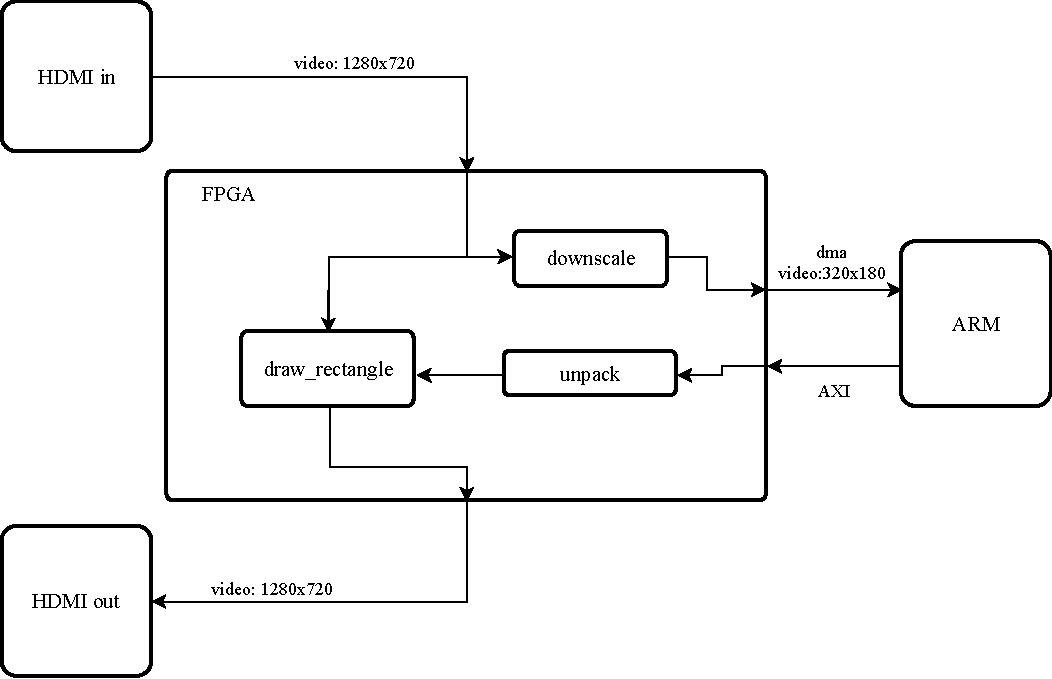
\includegraphics[width=0.68\textwidth]{resources/BlockDiagram-Original.pdf}
    \caption{Block diagram illustrating the original proposed design}
    \label{fig:blockdiagramFPGA-original}
\end{figure*}

\begin{figure*}[h!]
    \centering
    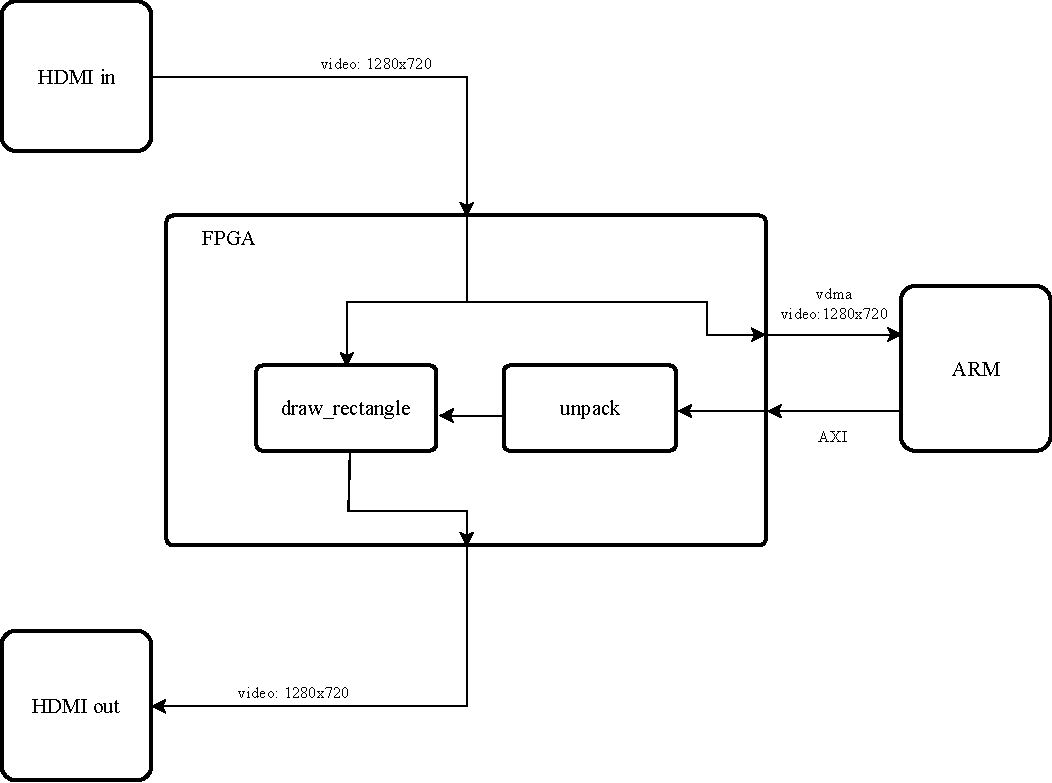
\includegraphics[width=0.68\textwidth]{resources/BlockDiagram-Revised.pdf}
    \caption{Block diagram illustrating the final implemented design}
    \label{fig:blockdiagramFPGA-revised}
\end{figure*}
\subsection{HLS code implementation details}
First of, all functionality is separated in functions. This does not only increase re-usability, readability and changeability but also helps the HLS tool to recognize parts which can be run in parallel. Secondly, opacity is taken into account and therefore slightly transparent rectangles can be drawn. Lastly, downscaling is performed completely independent of the other algorithms which will draw the rectangles and output the pixel. Down scaling saves a line of the current averages so every 16 pixel square can be averaged into one final pixel and written to the framebuffer. Do note however, that in the current version the downscaling is made inactive as elaborated in the previous section.

\subsection{downscale}
To reduce the burden of the ARM CPU, and thereby increasing overall performance, the down scaling should be performed on the FPGA in hardware. Using dedicated hardware, the down scaling can moreover be performed much more efficiently. We implemented the down-scaling on the FGPA including a double frame-buffer. This way we would be writing to one buffer while the other would be available for reading. Since these buffers would be one-fourth the size of the full frame, a double buffer would fit on the FPGA if we only store the 24-bit with actual color. In the end the DMA module refused to work and the documentation was slightly lacking from Xilinx's side so in the final design the applicable module is commented out.

\begin{table}[h]
    \centering
    \begin{tabular}{lrp{5.5cm}}
        \toprule
        \textbf{Value} & \textbf{Bits} & \textbf{Notes} \\
        \midrule
        idx & \numrange{175}{160} & Big-endian \\
        - & \numrange{159}{112} & 48-bit padding \\
        \midrule
        - & \numrange{111}{97} & 15-bit padding \\
        is\_on & \num{96} & Single draw enable bit \\
        ah & \numrange{95}{80} & Big-endian, converted using ah2argb, alpha \& hue \\
        x0 & \numrange{79}{64} & Big-endian, coordinate \\
        y0 & \numrange{63}{48} & Big-endian, coordinate \\
        x1 & \numrange{47}{32} & Big-endian, coordinate \\
        y1 & \numrange{31}{16} & Big-endian, coordinate \\
        s & \numrange{15}{0} & Big-endian, stroke thickness \\
        \bottomrule \\
    \end{tabular}
    \caption{Command layout, total data size including padding is \num{176} bits.}
    \label{tab:command-layout}
\end{table}

\subsection{unpack}
\label{ssec:unpack}
Data transfer transactions on AXI-lite between the FPGA and the main CPU is fairly slow. This makes the difference between for example 5 rectangle updates per second and 10 rectangle updates per second, for respectively 8 rectangle draw-commands or 1 rectangle draw command. Note that these commands only update the registers that the hardware uses to draw the rectangles, not draw the rectangle themselves. To reduce the impact the data transfer has on the framerate, data is packed on the CPU and unpacked on the FPGA, so the data for one rectangle can be written in one transaction, layout is shown in \cref{tab:command-layout}, in the transaction another 16 bits are appended for padding to a multiple of 4 bytes. As part of the command processing the alpha and hue values in the command is converted to ARGB in the hardware.

\subsection{draw rectangle}
The draw\_rectangle aims to draw a rectangle in certain positions, with certain visual settings, on the output video. It requires two coordinates and information about the color and opacity. The draw\_rectangle component can be used in parallel to draw multiple rectangles on the screen. As long as the FPGA has enough free resources, many rectangles, with different visuals, can be drawn at the same time without limiting the total pixel throughput.

\section{Measurements}
The python program measures the time between the face detection updates and calculates an FPS value. A multiple of these values are used to find an average. After this, three different scenarios are used to find the effectiveness of using a FPGA for certain tasks.

\subsection{Measurement 1}
For this measurement we used the BaseOverlay and the full frame to do face recognition, the ARM CPU was used to draw the rectangles. Due to the relative high resolution, the face detection for people which are some distance away was very good.
The performance however was abysmal, reaching just \SI{0.526}{\fps}, making the implementation completely unusable in any real time application. Moreover, during this measurement only one rectangle was drawn.

\subsection{Measurement 2}
%/3.5 to 5 FPS for optimized CPU (background same)
For this measurement we still used the BaseOverlay and the full frame was still sent to the CPU, also the rectangles were still drawn by the ARM CPU. However, only 1/4th of the resolution was used to do face recognition. This obviously resulted in a reduced face recognition accuracy but the performance also increased by a lot. This new implementation reached \SIrange{3.5}{5.1}{\fps}, making the implementation still very hard to use for real-time applications. The range is caused by drawing between 8 and 1 rectangles respectively.

\subsection{Measurement 3}
\label{ssec:measurement-3}
The final implementation moves the main compositing of the rectangle indicators and the image to the FPGA fabric, enabling a full framerate pass-through of the analyzed footage. Due to not having to output the frame over VDMA and not having to draw the rectangles, the face recognition performance saw a performance increase too, reaching \SIrange{4.5}{9.8}{\fps} for the hybrid implementation. The added benefit is that this implementation supports alpha blending, which OpenCV can also support but that would result in an even bigger performance cost. The main bottleneck with this implementation is the AXI-lite communication, as has already been outlined in \cref{ssec:unpack}.

\section{Conclusion}
As discussed and shown in \cref{ssec:unpack} and \cref{ssec:measurement-3}, the main performance bottleneck in the final implementation is the AXI-lite communication. For now, our best implementation, the hybrid solution, achieved the full throughput of \SI{60}{\fps} with the facial recognition updating the rectangles at \SIrange{4.5}{9.8}{\fps}. The next speed-up would be attained by removing the now serial interface with one port for all rectangles with an index, and moving to one port per draw rectangle. Do note that this is obviously much less scalable for higher number of rectangles. For that, one would need to use a DMA IP block to move a larger buffer with data to the hardware faster. Overall, the FGPA fabric shows it's great potential in handling parallel tasks and high throughput data streams, and also shows it's weakness in tooling, usability and control IO speed. Vivado HLS and the Pynq platform especially are designed to be easy to use for non-hardware designers, but as soon as you need anything from Vivado HLx that initial value proposition is completely gone.

% trigger a \newpage just before the given reference
% number - used to balance the columns on the last page
% adjust value as needed - may need to be readjusted if
% the document is modified later
%\IEEEtriggeratref{8}
% The "triggered" command can be changed if desired:
%\IEEEtriggercmd{\enlargethispage{-5in}}

% references section

\printbibliography

% that's all folks
\end{document}
